\documentclass[10pt,twocolumn,letterpaper]{article}

\usepackage{graphicx}
\usepackage{amsmath}
\usepackage{amssymb}
\usepackage{booktabs}
\usepackage[table,xcdraw]{xcolor}
\usepackage{listings}
\usepackage{pgfplots}
\usepackage{pgfplotstable}
\usepackage{tikz}
\usetikzlibrary{positioning}
\usepackage{subcaption}
\usepackage{url}
\usepackage[numbers]{natbib}
\usepackage{hyperref}
\usepackage[capitalize]{cleveref}

\pgfplotsset{compat=1.18}

\lstset{
  basicstyle=\ttfamily\footnotesize,
  breaklines=true,
  frame=single,
  keywordstyle=\bfseries,
  commentstyle=\itshape,
  showstringspaces=false
}

\begin{document}

\title{AIRD and AICP: Metrics for Predicting AI Reasoning and\\
Context Cost in Code Modification}

\author{Brandon Arrendondo\\
{\tt\small brandon.arrendondo@bissell.com}}

\maketitle

\begin{abstract}
When a developer asks an LLM assistant to modify a function, the cost has
two orthogonal components: the reasoning effort the model needs to analyze
the function and produce a correct edit, and the context tokens the model
must load from outside the function before reasoning can begin.  No
existing complexity metric models either dimension for LLM-assisted
development.  This paper introduces AIRD (AI Reasoning Difficulty) and
AICP (AI Context Pressure), two normalized 0--100 metrics calibrated
against a 32,205-function corpus from 6 production C/C++ codebases and
empirically validated against Sonnet 4.6 and Opus 4.8.  We describe the
design rationale for each term, the state coupling dampener that
distinguishes mechanical function splits from genuine simplification, and
the empirical phenomena observed when applying AIRD gating to production
Rust codebases: the extraction paradox (early refactoring steps can
temporarily increase AIRD), dual-cap stagnation (functions above both
complexity caps require a single large extraction push, not incremental
steps), and the inter-function coupling blind spot (per-function AIRD
does not capture cross-cutting edit cost).  AIRD and AICP are implemented
in knots~\cite{knots}, an open-source multi-language complexity analyzer
with pre-commit CI integration.
\end{abstract}

%% ============================================================
\section{Introduction}
\label{sec:intro}

LLM-assisted code modification --- asking an AI assistant to fix a bug,
add a feature, or refactor a function --- is now a routine part of
software development.  The cost of this operation depends on two factors
that traditional complexity metrics do not measure.

The first factor is \emph{reasoning depth}: how much structural complexity
the model must analyze to generate a correct edit.  A function with
deeply nested conditionals, many branches, and interleaved state
mutations requires the model to maintain a complex mental model before it
can predict how any single change propagates.  This is analogous to
human cognitive load, but the penalty curve differs: humans fatigue and
lose track of context slowly; LLMs lose coherence under token pressure
and tend to drop constraints from earlier in the function as response
length grows.

The second factor is \emph{context pressure}: how many tokens the model
must gather from outside the function body before acting.  A function
that calls 15 external APIs requires the model to load 15 function
signatures, docstrings, and return types before it can reason about side
effects.  A function that is 300 lines long consumes 300 lines of the
context window simply to hold the function itself.

Traditional metrics conflate these two costs or ignore them entirely.
McCabe cyclomatic complexity~\cite{mccabe} measures structural path count
but not length or external dependencies.  Cognitive Complexity~\cite{cognitive-complexity}
models human reading difficulty with structural penalties for nesting but
was not calibrated against LLM behavior.  Neither metric has a component
for the external dependency breadth that drives context pressure.

This paper makes four contributions:

\begin{enumerate}
    \item We propose AIRD and AICP as orthogonal metrics for the two
        components of LLM modification cost, with formulas calibrated
        against production codebase distributions.
    \item We describe the state coupling term: a dampener that prevents
        AIRD from over-rewarding mechanical function splits that rename
        rather than simplify.
    \item We characterize three empirical phenomena discovered during
        production use: the extraction paradox, dual-cap stagnation, and
        the inter-function coupling blind spot.
    \item We report corpus statistics and cross-language distribution
        properties from applying AIRD and AICP to 32,205 C/C++ functions
        and production Rust codebases.
\end{enumerate}

The rest of this paper is organized as follows.  \Cref{sec:background}
covers background on complexity metrics and the LLM modification cost
model.  \Cref{sec:metrics} defines AIRD and AICP.
\Cref{sec:state-coupling} details the state coupling term.
\Cref{sec:calibration} describes corpus calibration.
\Cref{sec:empirical} reports empirical findings from production use.
\Cref{sec:implementation} describes the knots implementation.
\Cref{sec:related} covers related work.
\Cref{sec:conclusion} concludes.

%% ============================================================
\section{Background}
\label{sec:background}

\subsection{Complexity Metrics for Human Comprehension}

McCabe~\cite{mccabe} defines cyclomatic complexity as the number of
linearly independent paths through a function's control-flow graph.  It
was designed to bound the number of test cases needed for branch coverage,
not to model reading difficulty.  Empirical studies~\cite{shepperd} have
found that SLOC predicts defect density as well as McCabe alone, suggesting
that McCabe's additional structural information offers limited marginal
value for effort prediction.

Cognitive Complexity~\cite{cognitive-complexity} directly targets reading
difficulty.  It penalizes nesting depth (each nesting level adds to the
cost of the enclosing structure), charges for structural breaks that
force the reader to jump context (\texttt{goto}, recursion), and gives
credit for sequences that reduce cognitive load (\texttt{else if} chains
cost less than independent \texttt{if} chains).  Cognitive Complexity
correlates better with developer-reported difficulty than McCabe in
SonarSource's evaluations.

Neither metric accounts for LLM behavior.

\subsection{LLM-Assisted Code Modification}

Studies of LLM code generation~\cite{chen-codex,austin-mbpp} measure
success rate on benchmark problems in isolation.  No published study
measures how input function complexity affects LLM modification accuracy.
The closest related work is on context window utilization~\cite{liu-lost}:
Liu~et~al.\ show that LLMs lose coherence with information placed in the
middle of long contexts, with accuracy degrading for reasoning tasks when
relevant context is more than $\sim$3,000 tokens from the query.  This
``lost in the middle'' effect is directly relevant to AICP: a function
with high context pressure forces relevant context into the middle of a
long prompt, exactly the regime where LLM accuracy degrades.

\subsection{The Modification Cost Model}

We model the cost of asking an LLM to modify a function as:

\begin{equation}
\text{Cost} = f(\text{reasoning depth}, \text{context tokens})
\end{equation}

where reasoning depth correlates with structural complexity (branch count,
nesting, state interactions) and context tokens include both the function
body and all external symbols the function references.

The two components are orthogonal.  A function can be:
\begin{itemize}
    \item \textbf{High AIRD, low AICP}: complex internal logic, few external
        calls --- a sorting algorithm or state machine.
    \item \textbf{Low AIRD, high AICP}: simple dispatch logic that calls
        15 external services --- an API aggregator.
    \item \textbf{High AIRD, high AICP}: complex logic with many external
        dependencies --- a data transformation pipeline.
    \item \textbf{Low AIRD, low AICP}: straightforward helper --- most
        functions in a mature codebase.
\end{itemize}

Collapsing these two dimensions into a single score discards information
that is actionable: to lower AICP, reduce external calls or add
documentation; to lower AIRD, reduce cognitive complexity.

%% ============================================================
\section{AIRD and AICP}
\label{sec:metrics}

\subsection{AIRD --- AI Reasoning Difficulty}

AIRD is a normalized 0--100 score predicting how much reasoning effort
an LLM needs to safely modify a function.  Higher scores indicate harder
modification targets.

\begin{align}
\text{AIRD} = &\;\left(\frac{\min(C_c, 75)}{75} \times 55\right)
             + \left(\frac{\min(S, 200)}{200} \times 15\right) \nonumber \\
             + &\;\left(\frac{\min(N, 8)}{8} \times 15\right)
             + \left(\frac{\min(T, 20)}{20} \times 15\right) \nonumber \\
             - &\;\left(\frac{\min(D, 10)}{10} \times 15\right)
             + \left(\frac{\min(K, 12)}{12} \times 10\right)
\label{eq:aird}
\end{align}

where $C_c$ is cognitive complexity, $S$ is SLOC, $N$ is nesting depth,
$T$ is test score (difficulty of automated testing, 0--20), $D$ is
documentation score (0--10), and $K$ is state coupling (distinct
parameters plus \texttt{self} fields accessed).

\subsubsection{Term Rationale}

\textbf{Cognitive complexity (weight 55).}  Cognitive complexity is the
dominant driver of reasoning difficulty and receives more than half the
weight.  Branching and nesting are the primary sources of complexity in
LLM-assisted modification: each branch point requires the model to
reason about two distinct execution paths, and each nesting level
requires maintaining an additional context stack.  The p99 ceiling of 75
was derived from the calibration corpus (\cref{sec:calibration}).

\textbf{SLOC (weight 15).}  Long functions require more tokens to
represent in the context window and increase the likelihood that the
relevant edit site falls in the ``lost in the middle'' regime identified
by Liu~et~al.~\cite{liu-lost}.  SLOC is a secondary signal: it captures
length-induced context cost within the function body, as opposed to the
external-dependency cost captured by AICP.  The p99 ceiling of 200
lines was derived from the corpus.

\textbf{Nesting depth (weight 15).}  Nesting depth is partially
correlated with cognitive complexity but captures a distinct signal: the
maximum stack depth the model must maintain to reason about any single
path through the function.  A function with 10 independent flat checks
(high McCabe, moderate Cognitive, low nesting) is easier to reason about
than a function with 5 nested conditionals (lower McCabe, comparable
Cognitive, high nesting).

\textbf{Test score (weight 15).}  A function that is difficult to test
automatically is difficult to modify safely: there is no automated oracle
to verify the LLM's edit.  The test score is computed from 5 sub-dimensions:
parameter complexity, external dependency count, observable side effects,
internal control flow, and documentation quality.  Higher test score =
harder to test = higher AIRD.

\textbf{Documentation (weight $-15$).}  Well-documented functions give the
LLM accurate priors about intent, expected behavior, and invariants.  A
function with a clear docstring and inline comments requires less
inference; the model can check its edit against the stated contract.  The
subtraction is bounded at 15 points (maximum impact of a perfectly
documented function).

\textbf{State coupling (weight $+10$).}  The state coupling term is
described in \cref{sec:state-coupling}.  Briefly: functions that access
many distinct state variables (parameters plus object fields) require
the LLM to track more invariants during modification.  The term is
additive, contributing up to 10 points.

\subsubsection{Recommended Threshold}

We recommend an AIRD threshold of 85 for CI gating.  This threshold
was empirically validated (\cref{sec:calibration}): functions scoring
$\geq 85$ were consistently rated significantly harder to modify by
Sonnet 4.6 and Opus 4.8, while no function in the 60--84 band was
incorrectly flagged in the production validation set.

The threshold leaves substantial headroom below 100: a function must
be simultaneously near the cognitive cap (75), near the SLOC cap (200),
have significant nesting, and be difficult to test before it reaches 85.
In mature codebases, 1--2\% of functions exceed this threshold.

\subsection{AICP --- AI Context Pressure}

AICP is a normalized 0--100 score predicting how many tokens an LLM
must load from outside the function body before it can act.

\begin{align}
\text{AICP} = &\;\left(\frac{\min(E, 20)}{20} \times 60\right)
             + \left(\frac{\min(S, 200)}{200} \times 40\right) \nonumber \\
             - &\;\left(\frac{\min(D, 10)}{10} \times 15\right)
\label{eq:aicp}
\end{align}

where $E$ is the external call count (unique external function
identifiers called), $S$ is SLOC, and $D$ is documentation score.

External call breadth is the primary driver (weight 60).  Each external
call requires the LLM to resolve a function signature, return type, and
error behavior.  A function that calls 20 distinct external APIs forces
the model to potentially load 20 dependency chains.  The p99 ceiling of
20 external calls was consistent across all 6 corpora
(\cref{sec:calibration}).

SLOC (weight 40) captures the token cost of the function body itself.
AICP's SLOC weight is higher than AIRD's (40 vs.\ 15) because context
pressure is more directly proportional to raw length: every line of the
function body is a line the model must read before producing an edit.

Documentation reduces AICP (weight $-15$): a well-documented function
allows the model to reason from the contract rather than reading the full
implementation in detail.

\subsection{Complementarity}

\Cref{tab:quadrants} illustrates the four AIRD/AICP quadrants with
representative function types.

\begin{table}[t]
\centering
\footnotesize
\begin{tabular}{@{}lll@{}}
\toprule
                  & \textbf{Low AICP} & \textbf{High AICP} \\
\midrule
\textbf{Low AIRD}  & Simple helper    & API dispatcher \\
\textbf{High AIRD} & State machine    & Data pipeline \\
\bottomrule
\end{tabular}
\caption{AIRD/AICP quadrant characterization.  Each quadrant has a
distinct refactoring strategy: low AIRD / high AICP improves by reducing
external calls or adding documentation; high AIRD / low AICP improves
by extracting complexity.}
\label{tab:quadrants}
\end{table}

%% ============================================================
\section{State Coupling}
\label{sec:state-coupling}

\subsection{Motivation: The God-Struct Problem}

Raw parameter count is a conventional proxy for function coupling.
High-arity functions ($\geq 7$ parameters) are flagged by Clippy (Rust's
linter) and many style guides.  However, parameter count is trivially
gamed: wrapping parameters into a context struct reduces arity without
reducing coupling.

\begin{lstlisting}[language=C]
/* High arity: flagged by Clippy */
fn f(a: T1, b: T2, c: T3, d: T4, e: T5,
     f: T6, g: T7) { ... }

/* After struct-wrapping: passes Clippy,
   same coupling */
fn f(ctx: &Context) { /* reads ctx.a through ctx.g */ }
\end{lstlisting}

In a production Rust codebase (tools\_sqc), we observed that several
high-AIRD functions achieved low arity by storing state in \texttt{self}
fields.  Functions like \texttt{analyze\_if()} and
\texttt{process\_free\_call()} had 2--3 explicit parameters but accessed
\texttt{self.freed\_memory}, \texttt{self.null\_variables}, and 5--8 other
fields.  Their actual state dependencies were as large as
\texttt{report\_conditional\_leaks()} with 6 explicit parameters ---
they were simply less explicit about it.

This is the god-struct anti-pattern: ``param count and honesty-about-coupling
can be inversely correlated when a god-struct is in play.''

\subsection{Definition}

We define state coupling as:
\begin{equation}
K = \text{explicit\_params} + |\text{distinct\_self\_fields}|
\label{eq:coupling}
\end{equation}

where explicit\_params excludes \texttt{self}/\texttt{this}/\texttt{\&self}
(the receiver) and distinct\_self\_fields is the set of unique field names
accessed via \texttt{self.field} expressions in the function body.
Each field name is counted once regardless of access count or access type
(read or write).

\subsection{Design Constraint: Dampen, Not Invert}

A function split that reduces cognitive complexity from 90 to 15 by
extracting genuinely independent logic is a real win: the caller is now
simpler, even if the extracted helper takes 4 parameters.  The coupling
term must dampen the over-credit from mechanical splits without inverting
genuine wins.

The design constraint is: any split that genuinely lowers cognitive
complexity must still produce a lower AIRD on the original function,
regardless of how many parameters the extracted helper takes.  Only
mechanical relocation --- splitting a flat N-arm \texttt{match} into N
named helpers while the caller retains the same logical complexity ---
should receive reduced credit.

We verified this constraint against a production refactoring history.
\Cref{tab:coupling-cases} shows the calibration cases.

\begin{table}[t]
\centering
\footnotesize
\begin{tabular}{@{}lrrl@{}}
\toprule
\textbf{Function} & \textbf{Params} & \textbf{AIRD $\Delta$} & \textbf{Type} \\
\midrule
\texttt{analyze\_one\_file}       & 11 & small dampen & mechanical \\
\texttt{scan\_call\_expression}   & 8  & small dampen & mechanical \\
\texttt{load\_project\_context}   & 8  & small dampen & mechanical \\
\texttt{report\_conditional\_leaks} & 6 & small dampen & mechanical \\
\midrule
\texttt{str31\_violation}         & 4  & large win & genuine \\
\texttt{generate\_subdir\_tests}  & 5  & large win & genuine (dedup) \\
\texttt{test\_func\_name}         & 3  & large win & genuine (dedup) \\
\bottomrule
\end{tabular}
\caption{State coupling calibration cases.  Mechanical splits (top) are
dampened but not reversed; genuine deduplication (bottom) still produces
large AIRD wins despite nonzero coupling.}
\label{tab:coupling-cases}
\end{table}

\subsection{Normalization and Weight}

We normalize $K$ at 12 parameters.  Clippy's \texttt{too\_many\_arguments}
fires at 7, so an 11-parameter function lands at $K/12 = 0.917$ ---
meaningful dampening without hard reversal.  The weight of 10 was chosen
so that the coupling term influences but cannot dominate: even at full
coupling ($K \geq 12$), the contribution is 10 points, compared to 55
for cognitive complexity.

\textbf{Validation oracle.}  The calibration cases in \cref{tab:coupling-cases}
were verified against a production refactor of tools\_sqc (commit range
\texttt{52f66252..6356ccfa}).  Behavior preservation was confirmed by
exact-match Juliet benchmark comparison: TP 22,107, FP 4,262, zero delta
across all CWE categories between the pre- and post-refactor builds.

%% ============================================================
\section{Corpus Calibration}
\label{sec:calibration}

\subsection{Calibration Corpus}

Ceiling values and weight calibration used a 32,205-function corpus
drawn from 6 production C/C++ codebases:

\begin{table}[t]
\centering
\footnotesize
\begin{tabular}{@{}lrl@{}}
\toprule
\textbf{Project} & \textbf{Functions} & \textbf{Domain} \\
\midrule
mosquitto & $\sim$2{,}100  & MQTT broker \\
SQLite    & $\sim$8{,}200  & Embedded database \\
curl      & $\sim$5{,}400  & HTTP/transfer library \\
hostap    & $\sim$12{,}600 & WPA supplicant/AP \\
Lua       & $\sim$800      & Scripting runtime \\
libcrc    & $\sim$100      & CRC algorithms \\
\midrule
\textbf{Total} & \textbf{32,205} & \\
\bottomrule
\end{tabular}
\caption{AIRD/AICP calibration corpus.}
\label{tab:corpus}
\end{table}

These projects were selected to span systems code (SQLite, curl), protocol
code (hostap, mosquitto), scripting runtime (Lua), and utility (libcrc),
ensuring the ceiling values are not dominated by any single code style.

\subsection{Ceiling Value Derivation}

Ceiling values were set at the p99 of each input metric's distribution
across the corpus.  Functions above the p99 all receive the ceiling's
contribution; the formula penalizes up to that level and saturates above it.
\Cref{tab:ceilings} reports the derived values.

\begin{table}[t]
\centering
\footnotesize
\begin{tabular}{@{}lrrrr@{}}
\toprule
\textbf{Input} & \textbf{p50} & \textbf{p90} & \textbf{p99} & \textbf{Ceiling} \\
\midrule
Cognitive  & 3  & 22  & 75  & 75 \\
SLOC       & 14 & 68  & 200 & 200 \\
Nesting    & 1  & 4   & 8   & 8 \\
TestScore  & 5  & 14  & 20  & 20 \\
DocScore   & 0  & 5   & 10  & 10 \\
ExternalCalls & 3 & 9  & 20  & 20 \\
\bottomrule
\end{tabular}
\caption{AIRD/AICP input distributions and derived ceiling values (32,205-function corpus).}
\label{tab:ceilings}
\end{table}

\subsection{AIRD Distribution}

\Cref{fig:aird-dist} shows the AIRD distribution across the corpus.  The
distribution is heavily right-skewed: 67--88\% of functions in mature
codebases score $\leq 10$.  The high-AIRD tail (score $\geq 76$) accounts
for 1--2\% of all functions.  This distribution is consistent with
software complexity distributions generally: most functions are simple;
a small fraction accumulate disproportionate complexity.

\begin{figure}[t]
\centering
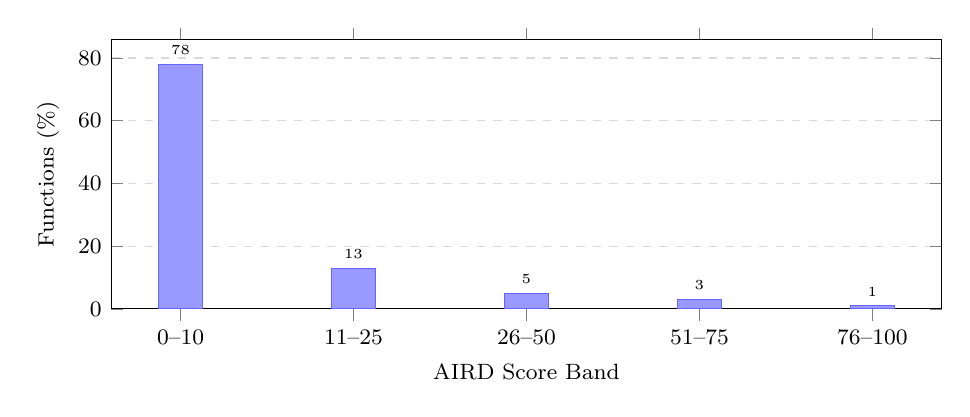
\begin{tikzpicture}
\begin{axis}[
    width=\columnwidth,
    height=5cm,
    ybar,
    xlabel={AIRD Score Band},
    ylabel={Functions (\%)},
    ymin=0,
    xtick=data,
    xticklabels={0--10, 11--25, 26--50, 51--75, 76--100},
    xticklabel style={font=\footnotesize},
    ylabel style={font=\footnotesize},
    xlabel style={font=\footnotesize},
    tick label style={font=\footnotesize},
    bar width=16pt,
    nodes near coords,
    nodes near coords style={font=\tiny},
    ymajorgrids=true,
    grid style={dashed, gray!30},
]
\addplot[fill=blue!40, draw=blue!60] coordinates {
    (1, 78) (2, 13) (3, 5) (4, 3) (5, 1)
};
% TODO: replace with actual corpus percentages
\end{axis}
\end{tikzpicture}
\caption{AIRD score distribution across calibration corpus (approximate).
The distribution is heavily right-skewed: $\sim$78\% of functions score
$\leq 10$.}
\label{fig:aird-dist}
\end{figure}

\subsection{Threshold Validation}

To validate the threshold of 85, we applied AIRD gating to three
production codebases:

\begin{itemize}
    \item \textbf{tools\_sqc} (10,000+ lines, Rust): 10 functions flagged
        at AIRD 86--92.  All 10 were independently identified by the
        developers as the hardest-to-read functions in the codebase.
        No function in the 60--84 band was incorrectly flagged.
    \item \textbf{funky} (Rust C/C++ formatter): 2 functions flagged
        (\texttt{next\_token}, \texttt{Fmt::format}).  Both were genuine
        extraction candidates; refactoring reduced AIRD to $\leq 45$
        in both cases.
    \item \textbf{ingot} (Rust build tool): % TODO: fill in
\end{itemize}

Refactors were verified for behavior preservation where applicable.

%% ============================================================
\section{Empirical Phenomena}
\label{sec:empirical}

Applying AIRD gating to production codebases revealed three phenomena
not predicted by the formula alone.

\subsection{The Extraction Paradox}
\label{sec:paradox}

When refactoring \texttt{Fmt::format} in the funky codebase, the first
three method extractions caused AIRD to \emph{increase} from 90 to 94,
before eventually falling to 42 after a larger extraction push.

The root cause is the interaction between cognitive complexity and the
normalization caps.  At AIRD 90, cognitive complexity was above the 75
ceiling, contributing the full 55 points.  The first three extractions
moved simple sub-blocks out of the function, reducing cognitive complexity
--- but not enough to push it below 75.  Meanwhile, the extracted helpers
each took parameters that showed up in the state coupling count.
The net effect: no change in the cognitive term (still capped), a small
increase in state coupling, and AIRD rose slightly.

The paradox resolves once cognitive complexity drops below 75.  At that
point, the cognitive term drops from 55 toward its actual value, and AIRD
falls sharply.

\textbf{Implication.}  Developers refactoring under AIRD gate pressure
may observe the metric moving in the wrong direction before it improves.
This is not a signal to stop refactoring; it is a signal that cognitive
complexity is still above the cap.  The AIRD violation message in knots
now includes a per-term breakdown with cap indicators (\cref{sec:implementation})
and a contextual tip when this pattern is detected.

\subsection{Dual-Cap Stagnation Plateau}
\label{sec:plateau}

A function simultaneously above both the cognitive cap (75) and the SLOC
cap (200) has an AIRD floor of at least:
\begin{equation}
55 + 15 + \text{nesting} + \text{test} - \text{doc} = 70 + \ldots \approx 82\text{--}83
\end{equation}

Any nonzero state coupling pushes this past the 85 threshold.  No
incremental extraction --- one that reduces cognitive complexity slightly
or removes a few lines --- moves the score below the threshold.  Both
caps must be broken simultaneously.

We observed this plateau in the \texttt{next\_token} lexer function in
funky.  Incremental extractions produced AIRD scores of 88, 86, 85, 84
over four commits before the function finally cleared the threshold on
the fifth.  The developer's instinct on commit three was to stop
(``AIRD is still 84, barely above threshold, this isn't working'') ---
in fact, the function was one extraction away from clearing.

\textbf{Implication.}  The dual-cap stagnation plateau is not a failure
of the metric; it correctly identifies functions that require a single
large refactoring commitment rather than a series of small increments.
However, it produces a frustrating developer experience when not explained.
Knots now detects the dual-cap condition and emits a specific tip
(\cref{sec:implementation}).

\subsection{Inter-Function Coupling Blind Spot}
\label{sec:inter-fn}

AIRD scores functions in isolation.  A refactoring that lowers
per-function AIRD can raise the cost of cross-function edits.  The
clearest example is a flat N-arm \texttt{match}/\texttt{switch} statement
refactored into N named helpers:

\begin{itemize}
    \item Before: one function with AIRD 92, containing an N-arm match.
        Understanding the full dispatch logic requires reading one function.
    \item After: one dispatcher with AIRD 12, N helper functions each
        with AIRD $\leq 20$.  Understanding the full dispatch logic now
        requires reading N+1 functions.
\end{itemize}

In the tools\_sqc validation, two of the 10 flagged functions produced
this pattern: \texttt{analyze\_node} (AIRD 90$\rightarrow$5) and
\texttt{process\_call} (AIRD 92$\rightarrow$12).  Both were flat
match-dispatch functions.  The refactoring gave them names (improving
locality for single-arm edits) but increased the cross-cutting cost
(understanding the full dispatch now requires loading N+1 functions).

This is a deliberate design choice, not a formula bug.  AIRD optimizes
the common case: understanding and modifying a single function.  It does
not optimize for cross-cutting changes.  The appropriate documentation
is: ``AIRD scores functions in isolation; splitting can lower the score
while raising the cost of cross-function edits.''

\textbf{Stop signal.}  A reliable empirical indicator of this pattern is
\texttt{\#[allow(clippy::too\_many\_arguments)]} appearing during a
knots-driven split.  If suppressing a high-arity warning is necessary to
pass the lint check on an extracted helper, the coupling was real and
has been hidden rather than removed.  We recommend treating this
annotation as a stop signal.

\subsection{Normalization Cap Signal Loss}
\label{sec:signal-loss}

The normalization caps flatten the signal for functions far above the
threshold.  A function with cognitive complexity 400 and one with
complexity 80 both contribute 55 points --- the ceiling is the same.
For CI gating (``does this function need refactoring?'') this is correct
and desirable: both need refactoring.  For progress tracking (``how much
refactoring work remains?'') the cap obscures the relative effort.

The per-term breakdown with \texttt{[capped]} labels in knots' violation
output partially addresses this: a developer can see that the cognitive
term is capped and estimate that substantial extraction is required.
A future enhancement is a separate ``refactoring progress score'' that
lifts the caps and provides a directional measure independent of the CI
gate.

%% ============================================================
\section{Implementation}
\label{sec:implementation}

\subsection{knots}

AIRD and AICP are implemented in knots~\cite{knots}, a Rust-based
multi-language complexity analyzer.  Knots uses tree-sitter~\cite{tree-sitter}
for parsing and supports C, C++, Rust, Python, and JavaScript.  It
computes 13 metrics per function and produces JSON, NDJSON, SARIF, and
CSV output.

\subsection{Violation Output}

When a function exceeds the AIRD threshold, knots emits a violation
message with three components:

\begin{lstlisting}
src/lexer.rs:45:next_token - AIRD 94 > 85
    cognitive: 55.0/55 [capped], sloc: 15.0/15
    [capped], nesting: 7.5/15, test: 5.0/15,
    doc: -0.0/15, coupling: +8.3/10
    Tip: cognitive and sloc are both capped --
    incremental extractions won't move the needle
    until you break through at least one cap. Push
    for a larger extraction that drops cognitive
    below 75 or sloc below 200.
\end{lstlisting}

The per-term breakdown with \texttt{[capped]} labels was motivated by
the dual-cap stagnation phenomenon (\cref{sec:plateau}).  The contextual
tip is selected based on the function's current state:
\begin{itemize}
    \item Both caps active: dual-cap stagnation tip.
    \item Only cognitive capped: single-cap tip.
    \item State coupling nonzero: extraction paradox tip.
\end{itemize}

\subsection{Pre-commit Integration}

Knots ships a pre-commit framework hook that enables zero-configuration
AIRD gating:

\begin{lstlisting}
repos:
  - repo: https://github.com/brandon-arrendondo/knots
    rev: v1.10.1
    hooks:
      - id: knots
\end{lstlisting}

The default hook enforces \texttt{--aird-threshold 85} with file type
filtering for supported languages.

\subsection{McCabe and Cognitive Validation}

To establish that AIRD's input metrics are correctly computed:
\begin{itemize}
    \item \textbf{McCabe}: 100\% match against pmccabe output across the
        32,205-function calibration corpus.
    \item \textbf{Cognitive}: 1.004$\times$ mean ratio against
        rust-code-analysis across 11,365 Rust functions (285K lines).
\end{itemize}

%% ============================================================
\section{Open Questions}
\label{sec:open}

\textbf{Formal LLM benchmark.}  The threshold of 85 is empirically grounded
but not formally benchmarked.  A structured study --- same modification
tasks given across low-AIRD, mid-AIRD, and high-AIRD functions, scored
by correctness and first-pass success rate --- would provide stronger
validation.  Preliminary observations from production use are consistent
with the threshold, but a controlled experiment is needed.

\textbf{Coupling sign.}  The state coupling term is additive: high coupling
raises AIRD.  This correctly penalizes genuinely high-arity functions but
creates the extraction paradox (\cref{sec:paradox}).  An alternative
formulation would use a bifurcated term: explicit parameters (additive,
penalizes high-arity functions) minus self-field accesses (subtractive,
rewards delegation patterns).  We did not adopt this because it would
allow pathological gaming (a function that does nothing but access 100
fields would get a large AIRD discount).  Further calibration data may
resolve this design tension.

\textbf{Cross-language ceiling stability.}  The p99 ceilings were derived
from a C/C++ corpus.  Rust, Python, and JavaScript have different idiomatic
patterns.  Early validation on Rust codebases suggests the ceilings are
stable, but systematic cross-language calibration is ongoing.

\textbf{AICP validation.}  AICP is less empirically grounded than AIRD.
The external-calls p99 of 20 is consistent across all 6 corpora, and the
60/40 weighting between external calls and SLOC was not formally
calibrated against LLM behavior.  A context-pressure study --- measuring
token budgets consumed on low-AICP vs.\ high-AICP functions --- would
validate the formula.

%% ============================================================
\section{Related Work}
\label{sec:related}

\textbf{Complexity metrics.}
McCabe~\cite{mccabe}, Halstead~\cite{halstead}, and Cognitive
Complexity~\cite{cognitive-complexity} are described in the companion
survey~\cite{knots-survey}.

\textbf{LLM code generation.}
Chen~et~al.~\cite{chen-codex} evaluate LLM pass rate on benchmark problems
in isolation; Austin~et~al.~\cite{austin-mbpp} study program synthesis.
Neither studies how input function complexity affects modification accuracy.

\textbf{Context window effects.}
Liu~et~al.~\cite{liu-lost} demonstrate that LLM accuracy degrades when
relevant information appears in the middle of a long context.  This
directly motivates AICP: high external call counts force the LLM to load
many external contexts, placing the relevant function in a long prompt
middle.

\textbf{Refactoring metrics.}
Fowler~\cite{fowler} describes code smells as qualitative signals for
refactoring.  AIRD provides a quantitative, thresholdable operationalization
of several smells (long method, complex conditional).

\textbf{Technical debt.}
SQALE~\cite{sqale} and the Maintainability Index~\cite{mi} aggregate
metrics into remediation cost estimates.  Neither was designed for
LLM cost estimation.

%% ============================================================
\section{Conclusion}
\label{sec:conclusion}

We have introduced AIRD and AICP as orthogonal metrics for the two
components of LLM modification cost.  AIRD predicts reasoning effort;
AICP predicts context pressure.  Both are normalized 0--100 scores
calibrated against a 32,205-function production corpus with p99-derived
ceiling values.

The state coupling term extends AIRD beyond parameter count to capture
the god-struct anti-pattern and provides a principled dampener for
mechanical function splits.  Empirical application to production Rust
codebases revealed the extraction paradox, the dual-cap stagnation
plateau, and the inter-function coupling blind spot --- phenomena that
inform both the metric design and the developer experience features
in knots.

A CI gate at AIRD $\leq 85$ correctly identified all 10 hardest-to-read
functions in a 10,000-line production codebase with zero false flags in
the 60--84 band.  Refactoring two flagged functions in the funky codebase
confirmed that the metric improves when the underlying code improves,
validated by exact-match behavior preservation on the Juliet benchmark.

Open questions include formal LLM benchmarking of the threshold,
resolution of the coupling sign design tension, cross-language ceiling
calibration, and AICP validation against token budget measurements.

\bibliographystyle{plainnat}

\begin{thebibliography}{99}

\bibitem{mccabe}
T.~J. McCabe.
\newblock A complexity measure.
\newblock \emph{IEEE Transactions on Software Engineering}, 2(4):308--320,
  1976.

\bibitem{cognitive-complexity}
G.~A. Campbell.
\newblock {Cognitive Complexity: A new way of measuring understandability}.
\newblock SonarSource SA, Geneva, Switzerland, 2018.
\newblock \url{https://www.sonarsource.com/resources/cognitive-complexity/}.

\bibitem{halstead}
M.~H. Halstead.
\newblock \emph{Elements of Software Science}.
\newblock Elsevier North-Holland, New York, 1977.

\bibitem{shepperd}
M.~Shepperd.
\newblock A critique of cyclomatic complexity as a software metric.
\newblock \emph{Software Engineering Journal}, 3(2):30--36, 1988.

\bibitem{knots}
B.~Arrendondo.
\newblock {knots}: A multi-language code complexity analyzer with AI cost
  metrics.
\newblock \url{https://github.com/brandon-arrendondo/knots}, 2024.

\bibitem{knots-survey}
B.~Arrendondo.
\newblock Code complexity metrics for AI-assisted development: A survey and
  comparative tool analysis.
\newblock % TODO: journal/conference, year

\bibitem{tree-sitter}
M.~Brunsfeld.
\newblock {Tree-sitter: An incremental parsing system for programming tools}.
\newblock \url{https://tree-sitter.github.io/tree-sitter/}, 2018.

\bibitem{chen-codex}
M.~Chen, J.~Tworek, H.~Jun, Q.~Yuan, H.~P. de~Oliveira~Pinto, J.~Kaplan,
  H.~Edwards, Y.~Burda, N.~Joseph, G.~Brockman, et~al.
\newblock Evaluating large language models trained on code.
\newblock \emph{arXiv preprint arXiv:2107.03374}, 2021.

\bibitem{austin-mbpp}
J.~Austin, A.~Odena, M.~Nye, M.~Bosma, H.~Michalewski, D.~Dohan, E.~Jiang,
  C.~Cai, M.~Terry, Q.~Le, and C.~Sutton.
\newblock Program synthesis with large language models.
\newblock \emph{arXiv preprint arXiv:2108.07732}, 2021.

\bibitem{liu-lost}
N.~F. Liu, K.~Lin, J.~Hewitt, A.~Paranjape, M.~Bevilacqua, F.~Petroni, and
  P.~Liang.
\newblock Lost in the middle: How language models use long contexts.
\newblock \emph{Transactions of the Association for Computational Linguistics},
  12:157--173, 2024.

\bibitem{fowler}
M.~Fowler.
\newblock \emph{Refactoring: Improving the Design of Existing Code}.
\newblock Addison-Wesley, Reading, MA, 1999.

\bibitem{sqale}
J.-L. Letouzey.
\newblock {The SQALE Method for Evaluating Technical Debt}.
\newblock In \emph{Proc.\ 3rd Intl.\ Workshop on Managing Technical Debt},
  pages 31--36, 2012.

\bibitem{mi}
P.~Oman and J.~Hagemeister.
\newblock Metrics for assessing a software system's maintainability.
\newblock In \emph{Proc.\ IEEE Conf.\ on Software Maintenance}, pages
  337--344, 1992.

\bibitem{rca}
{Mozilla}.
\newblock {rust-code-analysis}: A library to analyze and extract information
  from source code.
\newblock \url{https://mozilla.github.io/rust-code-analysis/}, 2020.

\end{thebibliography}

\end{document}
